
\chapter{Paper 4}\label{sc:p4}
\textbf{\Large 0.8V 1GHz Dynamic Comparator In Digital 90nm CMOS
  Technology}\\
%\newline
\indent   Carsten Wulff and Trond Ytterdal\\
\indent In proceedings of the 23rd NORCHIP Conference, 2005. \\
\indent 21-22 Nov. 2005 Pages 237 - 240 \\
\indent Digital Object Identifier: 10.1109/NORCHP.2005.1597033\\

\renewcommand\myfigname{p1fig:}
\renewcommand\myeqname{p1eq:}

\section*{Errata}
\begin{itemize}
\item Section 7.2, second paragraph, third sentence: What way
  $\rightarrow$ Which way
\item Section 7.3, fifth paragraph, second sentence: to threshold
  $\rightarrow$ to the threshold
\end{itemize}

%\textbf{Abstract:}
\begin{abstract}
The design of a 0.8V 1GHz dynamic comparator in digital 90nm
CMOS technology is presented. The work will show that low voltage, low
power and high speed analog circuits are feasible in nano-scale CMOS
technologies. The dynamic comparator dissipates a maximum of
222\begin{math}\mathrm{\mu}\end{math}W at 1GHz clock frequency with
100fF capacitive load and 0.8V supply voltage. This is lower than
comparable results. 
\end{abstract}


\section{Introduction}

One of the factors driving the downscaling of CMOS technology is the
ever present drive for price-per-performance of digital circuits. The
minimum dimensions get smaller and maximum supply voltages are reduced
due to reliability issues \cite{iwai99}.
%[1]
Since digital circuits are the driving force of silicon technology,
analog circuit designers often have to work in digital CMOS processes.
The reduction in supply voltage is not necessarily followed by an equal
reduction in threshold voltage, which limits the available voltage
headroom \cite{annema05}. 
%[2]
These nano-scale CMOS technologies offer many challenges that have
been discussed in previous publications, among others \cite{iwai99,annema05,annema04}.
%[1-3]
The challenges have, in some cases, brought success to simpler
topologies \cite{draxelmayr04}
%[4]
that have shown some of the advantages of nano-scale CMOS for analog
circuits. One advantage of scaling down is the increased speed that
follows. It can be shown that the unity gain frequency
(\textit{f$_{UG}$}) of a transistor is proportional to the effective
gate voltage (\textit{V$_{GT}$}) over the square of the length
(\begin{math}L\end{math}) of a transistor as given by (\ref{p1eq1})
%(1)
\cite{annema05}
%[2]
\eqn{
\label{p1eq1}
  f_{UG} \propto \dfrac{V_{GT}}{L^2}
}

Thus the trend will be that shorter lengths bring higher speeds.

Dynamic comparators are a class of circuits often used in pipeline
analog to digital converters (ADCs) \cite{cho95}.
%[5]
 As the name suggests a pipeline ADC consists of multiple stages. It
is common to extract at least 1.5-bits in each stage. The 1.5-bits per
stage stem from a digital error correction algorithm that requires a
certain redundancy in the number of bits. With the digital error
correction comparators in each stage can have quite large offset. Using
1.5-bits per stage one can tolerate a comparator offset of up to
\begin{math}\pm{}\end{math}V$_{REF}$/4, where V$_{REF}$ is the high
reference voltage minus the common mode voltage. In general, the
comparators can tolerate an offset up to
\begin{math}\pm{}\end{math}V$_{REF}$/2$^{b}$ for a b-bit stage
\cite{sumanen00}.
%[6]
Using dynamic comparators may reduce the architectural complexity
and reduce power dissipation, but tight control over variations and
mismatch must be exercised to ensure that offset and other errors are
kept within the allowed limits. Architectures that reduce mismatch have
been presented \cite{sumanen00}.
%[6]
In this paper, we describe a dynamic comparator that is a
modification of MOSFET-only fully-differential dynamic comparator
presented in \cite{lofti03}.
%[7]
 We will first describe the architecture and operation of the
comparator before we present the design in 90nm CMOS and simulation
results.
 

\section{Dynamic comparator architecture}

The circuit can be seen in Figure \ref{p1fig:dccomp}. In \cite{lofti03}
%[7]
they used a clock booster to supply a higher voltage to M1-M4 than
the supply voltage. To avoid any reliability concerns that may come
with boosted voltages we have replaced the clock booster with a single
transistor M5. The comparator has two phases; Reset and Latch. In the
Reset phase the latch, shown by the back to back inverters, is shorted
to ground through M6 and M7. To stop current flowing through the
shorted inverters M5 is turned off. Notice that both operations are
accomplished by a transition on CLK from low to high. This resets the
output of the comparator to zero and place INV1 and INV2 in a known
state. For the comparator to work properly it is important that INV1
and INV2 are reset to a known state, any unintentional imbalance
between the two inverters might tip the comparator towards one side.
 
When the clock goes from high to low we enter the Latch phase. In this
phase the inverters are connected in a positive feedback loop. What way
the latch will swing is controlled by an intentional imbalance in the
supply to the inverters. This imbalance is controlled by the
transistors M1-M4. Depending on their gate voltages transistors M1-M4
have variable on-resistance. For the moment we will ignore transistors
M2 and M3. If M1 and M4 are matched, their on-resistances will be the
equal when the differential input voltage (V$_{INPUT}$) is zero (VIN =
VIP). When V$_{INPUT}$ is negative (VIN \begin{math}>\end{math} VIP) M4
will turn more off, and the resistance in M1 will be lower than
resistance in M4. Thus INV1 will be slightly faster than INV2, and the
comparator will settle to VOP equals zero and VON equals one. The
opposite will occur if the V$_{INPUT}$ is positive (VIP
\begin{math}>\end{math} VIN). Notice that this comparator does not need
multiple clocks or inverted clocks, one clock signal is sufficient to
trigger transition from one phase to another and back again.
 

\begin{figure}[htbp]
\centerline{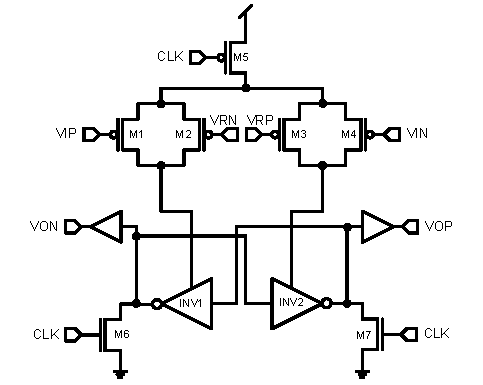
\includegraphics[width=\myfigwidth]{img0}}
  \caption{Dynamic comparator}
  \label{p1fig:dccomp}
\end{figure}

As stated, with M2 and M3 ignored the comparator has a threshold at
V$_{INPUT}$ = 0. However, in a 1.5-bit pipeline stage we need two
comparators with the thresholds given by eqs. (\ref{p1eq2})
and (\ref{p1eq3}) \cite{sumanen00}.  The transistors M2 and M3 serve to offset the threshold of the
comparator. They add small amounts of current to the two branches and
intentionally tip the balance of the comparator. Ideally we would scale
M2 and M3 to one fourth of the width of M1 and M4. However, as we will
se later, this is different in a real process.
 
\eqn{
\label{p1eq2}
V_{INPUT} = + \frac{1}{4}V_{REF}
}
\eqn{
\label{p1eq3}
V_{INPUT} = - \frac{1}{4}V_{REF}
}


We have two reference voltages, high and low. These are common mode
plus V$_{REF}$ and common mode minus V$_{REF}$, respectively. With the
high and low reference voltages connected to VRP and VRN, respectively,
the threshold will be set at (\ref{p1eq2})
%(2)
. If we reverse the connections to VRP and VRN we set the threshold at
(\ref{p1eq3})
%(3)
.
 


The boundary conditions for the inverters play an important role in
deciding which way the comparator swings. If we have large difference
in e.g. the capacitive load at the output of the inverters the
comparator might swing the wrong way. Therefore, we keep the load
controlled by using two matched buffers at the output of the inverters.
We have chosen a high reference at 0.6V and a low reference at 0.2V.
The common mode is set at 0.4V. Thus, the maximum allowable offset in
this work is \begin{math}\pm{}\end{math}V$_{REF}$/4 =
\begin{math}\pm{}\end{math}0.2V/4 = \begin{math}\pm{}\end{math} 50mV.
Simulations will show that the comparator stays within this limit.
 

Mismatch between transistors can influence the offset of the
comparator. Mismatch of MOSFET transistors can be reduced by increasing
the area of the transistor \cite{pelgrom89}. We tried to keep transistor areas as large as possible in order to
reduce mismatch, while small enough to keep capacitances low. All
transistors have a length of 0.1\begin{math}\mathrm{\mu}\end{math}m to
maximize the speed, according to (\ref{p1eq1}). All PMOS devices have a width of
3\begin{math}\mathrm{\mu}\end{math}m and all NMOS devices have a width
of 1.2\begin{math}\mathrm{\mu}\end{math}m as seen in Table \ref{p1tab:p1_widths}. Devices are kept
at the same width to simplify layout to maximizing the matching
\cite{johns}. Notice that the effective width, width x Number of Unit Devices in
parallel (NUD), of M1 and M2 does not correspond to a scaling of
one-fourth.  In the 90nm process we are using a scaling of eight was
necessary to keep the threshold at the reasonable level. M6 and M7 are
the twice the effective width of the NMOS transistors in the inverters.

\begin{table}[htbp]
\centering
\renewcommand{\arraystretch}{1.3}
\caption{ Transistor widths and fingers. $^{1}$NUD:  Number of Unit Devices in parallel }
\label{p1tab:p1_widths}
\begin{tabular}{l|l|l}
\hline
\textbf{Transistor}&\textbf{Width (\begin{math}\mathrm{\mu}\end{math}m)}&\textbf{NUD$^{1}$} \\
\hline
M1 \& M4 & 3.0
&
16
 \\
\hline
M2 \& M3
&
3.0
&
2
 \\
\hline

M5
&
3.0
&
84
 \\
\hline
M6 \& M7
&
1.2
&
2
 \\
\hline
\end{tabular} 
\end{table}

 

\section{Simulation Results}

Some of the key parameters for this dynamic comparator are offset,
delay and power dissipation. The offset needs to be within plus/minus
one-fourth of the reference voltage, which in our case corresponds to
\begin{math}\pm{}\end{math}50mV. We aimed for a speed of 1GHz at 0.8V.
This corresponds to a maximum delay of 500ps from CLK goes low to
output is valid. Remember that the comparator has two phases; Reset and
Latch, they need 500ps each at 1GHz clock frequency with a 50\% duty
cycle. We have not considered other duty cycle arrangements.

Since we were primarily considering high speed and low voltage, we did
not set any requirements for power dissipation. However, dynamic
comparator power dissipation resembles that of digital gates, which
have a power dissipation given approximately by:

\eqn{
\label{p1eq4}
  P = f C V_{DD}^2 + V_{DD}I_0
}

Where \begin{math}f\end{math} is the output frequency,
\textit{V$_{DD}$} is the supply voltage, \begin{math}C\end{math} is the
output capacitance and \textit{I$_{0}$} is the average leakage current
\cite{vittoz94}
%[10]
. With a low supply voltage and limited capacitance we anticipated
reasonable power consumption.


Simulations were performed in five process corners; Fast, Typical,
Slow and cross corners (fast NMOS, slow PMOS and visa versa). We also
ran three temperature corners (-40$^{o}$, 0$^{o}$, 85$^{o}$) for each
process corner. In addition, Monte Carlo simulations were performed to
simulate the effect of mismatch. All transistors included a model of
gate leakage current. A capacitive load of 100fF was used at the output
of the buffers in all simulations. Each parameter (offset, delay and
power dissipation) was extracted in each of the corners. Typical values
were extracted from typical process corner. The standard deviation
(\begin{math}\sigma{}\end{math}) for power dissipation and offset was
extracted from a Monte Carlo simulation. For offset it was around 3 mV
for both high and low threshold. For power dissipation the standard
deviation was negligible. We subtracted 3\begin{math}\sigma{}\end{math}
from the minimum value and added 3\begin{math}\sigma{}\end{math} to the
maximum value of offset and power dissipation. Table \ref{p1tab:p1_offset} shows the
results for comparator offset and power dissipation including
3\begin{math}\sigma{}\end{math}.  The offset is within
\begin{math}\pm{}\end{math}25mV which is well below the required
\begin{math}\pm{}\end{math}50mV. The maximum power dissipation was
222\begin{math}\mathrm{\mu}\end{math}W, almost half of this was
dissipated in the output buffers. As previously stated we have used a
similar architecture to that of \cite{lofti03}. They achieved 100\begin{math}\mathrm{\mu}\end{math}W with 200fF at
50Msamples/s and 1V in a 0.25\begin{math}\mathrm{\mu}\end{math}m CMOS
technology. Since most of the power dissipation in this architecture is
dynamic we can use (\ref{p1eq4})
to compare the two results.  If we scale the results from \cite{lofti03}
to 1GHz with 100fF and 0.8V we get a power dissipation of
640\begin{math}\mathrm{\mu}\end{math}W. Thus, a maximum power
dissipation of 222\begin{math}\mathrm{\mu}\end{math}W at 1GHz with
100fF and 0.8V can be considered reasonable.
 


Simulating delay in a comparator requires that one choose the input
signal with care. It can be shown that the delay of latched comparators
becomes large when the differential input voltage is close to threshold
\cite{johns}. We simulated the delay around the threshold by applying a
differential ramp at the input from 20mV above the ideal threshold to
20mV below the ideal threshold using 200 clock periods running at 1GHz.
The change in input from one clock period to the next was around
200\begin{math}\mathrm{\mu}\end{math}V. It is difficult to know exactly
where the threshold of the comparator is. We therefore used the delay
of the second pulse after the comparator switched states. By doing this
we know we never measure delay exactly at the threshold, but always
within 200\begin{math}\mathrm{\mu}\end{math} -
400\begin{math}\mathrm{\mu}\end{math}V away from the threshold. As with
offset and power dissipation, a Monte Carlo simulation was performed to
get the \begin{math}\sigma{}\end{math} of the delay. The
\begin{math}\sigma{}\end{math} of the delay decreased as we moved away
from the threshold. The standard deviation of the delay for the first
pulse after threshold was up to 30-50ps for high and low thresholds,
most of which we believe is due to varying distance to threshold when
the comparator latches. The \begin{math}\sigma{}\end{math} of the delay
for the second pulse was below 10ps, it is this
\begin{math}\sigma{}\end{math} that has been used in Table  \ref{p1tab:p1_offset}. In the
worst corner and including 3\begin{math}\sigma{}\end{math} variation in
delay due to mismatch, the comparator has less than 400ps delay. This
would give us a maximum clock frequency of 1.25GHz, but allowing for a
safety margin we choose 1GHz as maximum.
 


If the differential input voltage is closer than
\begin{math}\pm{}\end{math}200\begin{math}\mathrm{\mu}\end{math}V to
the threshold, less than what was used in simulation, there is a chance
of metastability. Metastability is when the comparator has larger delay
than the available settling time. A detector for metastability can be
inserted after the comparator \cite{kinniment99}. A XOR port connected to VON and VOP, with delay much smaller than
the comparator, will give a one if there is no metastability and zero
if there is metastability. This is ensured by the reset to zero of both
outputs in the Reset phase. In a case of metastability one can
arbitrarily choose output state of the comparator since one knows that
the input is close to threshold, much closer than the required
\begin{math}\pm{}\end{math}50mV. However, when using a metastability
detector one must make sure that the pull-down delay of Reset plus
delay of the detector is less than half the clock period. In this
design the pull-down delay in Reset was below 200ps. We have not yet
considered effects of layout parasitics.
 

\begin{table}[htbp]
\centering
\renewcommand{\arraystretch}{1.3}
\caption{ Offset, power dissipation and delay}
\label{p1tab:p1_offset}
\begin{tabular}{l|l|l|l|l}
\textbf{Parameter}
&
\textbf{Min}
&
\textbf{Typ}
&
\textbf{Max}
&
\textbf{Unit}\\
\hline

Offset (High threshold)
&
-22.5
&
9
&
15
&
mV
 \\
\hline
Offset (Low threshold)
&
-16
&
8.5
&
22
&
mV
 \\
\hline
Power diss.@1GHz
&
180
&
193
&
222
&
\begin{math}\mathrm{\mu}\end{math}W
 \\
\hline
Delay
&
80
&
186
&
\begin{math}<\end{math} 400
&
ps
 \\
\hline
\end{tabular}
 
\end{table}

\section{Future work}

The comparator is scheduled for production in a digital 90nm CMOS
technology during fall of 2005. The main purpose of the prototype is to
verify the rather small variations due to process variation and
mismatch seen in simulations. If the prototype confirms what has been
seen in simulations the comparator will be used in scheduled high
performance ADCs.
 

\section{Acknowledgements}
Financial support from the Norwegian Research Council through the
project Smart Microsystems for Diagnostic Imaging in Medicine (project
number 159559/130) and the project ASICs for Microsystems (project
number 133952/420) is gratefully acknowledged.
 

\section{Conclusion}
The design of a 0.8V 1GHz dynamic comparator in digital 90nm CMOS
technology has been presented. The work shows that low voltage, low
power and high speed analog circuits are feasible\textit{ }in
nano-scale CMOS technology. The dynamic comparator dissipates a maximum
of 222\begin{math}\mathrm{\mu}\end{math}W at 1GHz clock frequency with
100fF capacitive load at a supply voltage of 0.8V which is lower than
comparable results. Table  \ref{p1tab:p1_summary} shows a summary of simulation results.
 
 



 



 



 



 
\begin{table}[htbp]
\centering
\renewcommand{\arraystretch}{1.3}
\caption{ Summary of simulation results}
\label{p1tab:p1_summary}
\begin{tabular}{l|l}
Offset
\begin{math}<\end{math} \begin{math}\pm{}\end{math} 25mV
 \\
\hline
Clock Frequency
&
\begin{math}>\end{math} 1GHz
 \\
\hline
Power dissipation
&
\begin{math}<\end{math} 222\begin{math}\mathrm{\mu}\end{math}W
 \\
\hline
Supply voltage
&
0.8 V
 \\
\hline
Clock signals
&
1
 \\
\hline
High reference
&
0.6V
 \\
\hline
Low reference
&
0.2V
 \\
\hline
Common mode
&
0.4V
 \\
\hline
\end{tabular}
\end{table}



 

%\section{References}



 

% \begin{enumerate}
% 	\item \styleReferences{Iwai, H.; \textquotedblleft{}CMOS technology-year
% 2010 and beyond \textquotedblleft{}. Solid-State Circuits, IEEE Journal
% of Volume 34,~ Issue 3,~ March 1999 Page(s):357 - 366}
% 	\item \styleReferences{Annema, A.J.; Nauta, B. ; van Langevelde, R.;
% Tuinhout, H.; \textquotedblright{}Analog Circuits in
% Ultra-Deep-Submicron CMOS\textquotedblright{}. IEEE Journal of Solid
% State Circuits, Vol 40. 1. January 2005. Pages: 133-143}
% 	\item \styleReferences{Annema, A.J.; Nauta, B.; van Langevelde, R.;
% Tuinhout, H.; \textquotedblleft{}Designing outside rails
% constraints\textquotedblright{}. IEEE Int. Solid-State Circuits Conf.
% (ISSCC) Dig. Tech. Papers, 2004, Pages: 134-135}
% 	\item \styleReferences{Draxelmayr, D; \textquotedblleft{}A 6b 600MHz 10mW
% ADC Array in Digital 90nm CMOS\textquotedblright{}. IEEE Int.
% Solid-State Circuits Conf. (ISSCC) Dig. Tech. Papers, 2004}
% 	\item \styleReferences{Cho,T.H.; Gray, P.R; \textquotedblright{}A 10 b, 20
% Msample/s, 35mW Pipeline A/D Converter\textquotedblright{}, IEEE
% Journal of Solid-State Circuits. Vol. 30. NO. 3. March 1995,
% Pages:166-169}
% 	\item \styleReferences{Sumanen, L.; Waltari, M.; Halonen, K.;
% \textquotedblleft{}A mismatch insensitive CMOS dynamic comparator for
% pipeline A/D converters \textquotedblleft{} Electronics, Circuits and
% Systems, 2000. ICECS 2000. The 7$^{th}$ IEEE International Conference
% on Volume 1,~ 17-20 Dec. 2000 Pages:32 - 35 vol.1}
% 	\item \styleReferences{Lofti, R; Taherzadeh-Sani, M; Yaser Azizi, M; Shoaei,
% O; \textquotedblleft{} A 1-V MOSFET-only fully-differential dynamic
% comparator for use in low-voltage pipelined A/D
% converters\textquotedblright{}, Signals, Circuits and Systems, 2003.
% SCS 2003. International Symposium on
% \\
% Volume 2,~ 10-11 July 2003 Page(s):377 - 380 vol.2}
% 	\item \styleReferences{Pelgrom, M.J.M.; Duinmaijer, A.C.J.; Welbers, A.P.G.;
% \textquotedblleft{}Matching properties of MOS
% transistors\textquotedblright{} Solid-State Circuits, IEEE Journal of
% Volume 24,~ Issue 5,~ Oct 1989 Page(s):1433 \textendash{} 1439}
% 	\item \styleReferences{Johns, D.; Martin, J.; \textquotedblleft{}Analog
% Integrated Circuit Design\textquotedblright{}. John Wiley \& Sons,
% Inc., 1997}
% 	\item \styleReferences{Vittoz,E.; \textquotedblleft{}Micropower
% techniques\textquotedblright{}. Design of VLSI circuits for
% Telecommunication and Signal Processing. Chapter 5, Prentice Hall,
% 1994}
% 	\item \styleReferences{Kinniment, D.J.; Yakovlev, A.V.;
% \textquotedblleft{}Low power, low noise micropipelined flash A-D
% converter\textquotedblright{}. Circuits, Devices and Systems, IEE
% Proceedings. Volume 146,~ Issue 5,~ Oct. 1999 Page(s):263 - 267}
% \end{enumerate}



 



  


%%% Local Variables: 
%%% mode: latex
%%% TeX-master: "tb_paper1"
%%% End: 
